\documentclass[output=paper,
colorlinks,
citecolor=brown,
newtxmath
]{langscibook}
\bibliography{localbibliography}

\title{Maximal interpretation and definiteness of nominal phrases in Russian: Implication for the NP/DP parameter}
\author{%
Takuya Miyauchi\affiliation{The University of Tokyo}\orcid{0000-0003-4836-1617}}
\abstract{
The aim of this paper is to demonstrate that the maximal (exhaustive) interpretation of nominal phrases cannot be used to support the existence of determiner phrases in Russian. The paper argues that the maximal interpretation of phrases including numerals and possessives arises irrespective of the syntactic position of the possessors. Rather, it should be dealt with as a merely semantic matter and the difference between the maximal and non-maximal interpretations can be reduced to (in)definiteness.

\keywords{Russian, maximal interpretation, definiteness, DP hypothesis, numeral, possessive}
}

% add all extra packages you need to load to this file

\usepackage{tabularx,multicol}
\usepackage{url}
\urlstyle{same}

\usepackage{listings}
\lstset{basicstyle=\ttfamily,tabsize=2,breaklines=true}

\usepackage{langsci-optional}
\usepackage{langsci-lgr}
\usepackage{langsci-gb4e}
\usepackage[linguistics]{forest}
\usepackage{setspace}
\usepackage{pifont}
\usepackage[normalem]{ulem}
\usepackage{tabto}

\usepackage{relsize}


\usepackage{multicol}
\usepackage{textgreek}

\newcommand*{\orcid}{}


% \IfFileExists{../localcommands.tex}{%hack to check whether this is being compiled as part of a collection or standalone
%   % add all extra packages you need to load to this file

\usepackage{tabularx,multicol}
\usepackage{url}
\urlstyle{same}

\usepackage{listings}
\lstset{basicstyle=\ttfamily,tabsize=2,breaklines=true}

\usepackage{langsci-optional}
\usepackage{langsci-lgr}
\usepackage{langsci-gb4e}
\usepackage[linguistics]{forest}
\usepackage{setspace}
\usepackage{pifont}
\usepackage[normalem]{ulem}
\usepackage{tabto}

\usepackage{relsize}


\usepackage{multicol}
\usepackage{textgreek}

%   \newcommand*{\orcid}{}

\togglepaper[10]
% }{}

\begin{document}
\shorttitlerunninghead{Maximal interpretation and definiteness of nominal phrases in Russian}
\maketitle

\section{Introduction}
The literature on the structure of Slavic nominal phrases without overt articles splits into two standpoints. Some researchers insist on the presence of determiner phrases (DPs) even in articleless Slavic languages (\textsc{Universal DP Hypothesis}; see, e.g., \citealt{Progovac1998,Rappaport2002,Rutkowski2002,Basic2004,Franks.Pereltsvaig2004, Pereltsvaig2007a,Rutkowski.Maliszewska2007}). Others maintain that nominal phrases in Slavic are NPs (\textsc{Parameterized DP Hypo\-thesis}; e.g., \citealt{Zlatic1998,Trenkic2004,Boskovic2005,Boskovic2007,Boskovic2009,Despic2013}). \citet{Kagan.Pereltsvaig2012} contributed to the investigation of this matter by considering some behaviors of adjectival modifiers. They conclude that the DP layer exists even in articleless Russian.

%    \largerpage % Necessary to have the whole of fn. 2 on the same page

The aim of the present paper is to demonstrate that a maximal (exhaustive) interpretation of nominal phrases cannot be used to support the claim that there is a DP projection in Russian. Contrary to \citet{Kagan.Pereltsvaig2012}, I claim that a maximal interpretation of phrases including numerals and possessors arises independently of the high syntactic position of the possessor, since it is also available with possessors in a low syntactic position. The maximal interpretation should thus be dealt with as a merely semantic matter. It follows that the difference between maximal and non-maximal interpretations can be reduced to an opposition of definiteness versus indefiniteness.

The paper is organized as follows: \sectref{FW} provides some data regarding a maximal interpretation in Russian nominal phrases with a focus on prenominal and postnominal possessors. In addition, I outline the discussion of \citet{Kagan.Pereltsvaig2012} in terms of a maximal interpretation. \sectref{AN} presents my hypothesis that the maximal interpretation can be reduced to simple definiteness on the basis of the semantics of definiteness. \sectref{secDE} and \sectref{secGN} verify the validity of the hypothesis by using the definiteness effect and the genitive of negation. \sectref{CON} concludes the paper.

\section{Russian possessors and their interpretation}\label{FW}
\subsection{Prenominal possessors}\label{PreP}

In Russian, adjectival modifiers such as possessive adjectives (like \textit{Dimin} `Dima's', \textit{Mašin} `Masha's') can precede or follow numerals as shown in \REF{Num-Poss} and \REF{Num-Poss2}.\footnote{In this paper, the focus is on possessives. In fact, some other adjectival modifiers seem to behave almost the same way as possessive adjectives in terms of word order (see \sectref{MS}). However, further research is necessary to draw conclusions about the correlation between syntactic positions of other adjectives and the rise of a maximal interpretation.}

\ea\label{Num-Poss}
\ea\label{NumPoss} \gll pjat' Diminyx knig\\
five Dima.\textsc{gen.pl} book.\textsc{gen.pl}\\
\glt `five of Dima's books'

\ex\label{PossNum} \gll Diminy pjat' knig\\
Dima.\textsc{nom.pl} five book.\textsc{gen.pl}\\
\glt `Dima's five books' \hfill \citep[173]{Kagan.Pereltsvaig2012}
\z\z

\ea\label{Num-Poss2}
\ea\label{NumPoss2} \gll devjat' Mašinyx sumok\\
nine Masha.\textsc{gen.pl} bag.\textsc{gen.pl}\\
\glt `nine of Masha's bags'

\ex\label{PossNum2} \gll Mašiny devjat' sumok\\
Masha.\textsc{nom.pl} nine bag.\textsc{gen.pl}\\
\glt `Masha's nine bags'
\z\z

\noindent The phrases \REF{NumPoss} and \REF{NumPoss2}, where the possessive adjectives follow the numerals, are not interpreted maximally: Dima may have more than five books, and Masha may have more than nine bags. These phrases show the unmarked word order, thus possessives in Russian are usually considered non-exhaustive \citep[see, e.g.,][]{Partee2006}. However, \citet{Kagan.Pereltsvaig2012} point out that the alternative order is possible where a possessive adjective precedes a numeral. For example, the phrases \REF{PossNum} and \REF{PossNum2} are grammatical. Unlike \REF{NumPoss} and \REF{NumPoss2}, the phrases in \REF{PossNum} and \REF{PossNum2} receive a maximal interpretation and presuppose that Dima has exactly five books and Masha has exactly nine bags, respectively.

The difference in interpretation is reflected in the contrast between \REF{NumPossALL}, \REF{NumPoss2ALL} and \REF{PossNumALL}, \REF{PossNum2ALL}, respectively.

\ea\label{Num-PossALL}
\ea[*]{\label{NumPossALL}
\gll vse pjat' Diminyx knig\\
all.\textsc{nom.pl} five Dima.\textsc{gen.pl} book.\textsc{gen.pl}\\
\glt Intended: `all five of Dima's books'}
\ex[]{\label{PossNumALL}
\gll vse Diminy pjat' knig\\
all.\textsc{nom.pl} Dima.\textsc{nom.pl} five book.\textsc{gen.pl}\\
\glt `all Dima's five books'}
\z\z

\ea\label{Num-Poss2ALL}
\ea[*]{\label{NumPoss2ALL}
\gll vse devjat' Mašinyx sumok\\
all.\textsc{nom.pl} nine Masha.\textsc{gen.pl} bag.\textsc{gen.pl}\\
\glt Intended: `all nine of Masha's bags'}
\ex[]{\label{PossNum2ALL}
\gll vse Mašiny devjat' sumok\\
all.\textsc{nom.pl} Masha.\textsc{nom.pl} nine bag.\textsc{gen.pl}\\
\glt `all Masha's nine bags'}
\z\z

\noindent The universal quantifier \textit{ves'} `all' compels the maximal interpretation because of its lexical meaning. Therefore, it can be added to \REF{PossNum} and \REF{PossNum2}, which receive the maximal interpretation without semantic contradiction as shown in \REF{PossNumALL} and \REF{PossNum2ALL}. However, it cannot be added to \REF{NumPoss} or \REF{NumPoss2}, which do not receive a maximal interpretation because of semantic contradiction as shown in \REF{NumPossALL} and \REF{NumPoss2ALL}.

The above-mentioned statements regarding possessive adjectives also apply to possessive pronouns (e.g. \textit{naš} `our', \textit{tvoj} `your') as shown in \REF{Num-Possprn} and \REF{Num-Possprn2}.

\ea\label{Num-Possprn}
\ea\label{NumPossprn}
\gll \minsp{(*} vse) pjat' našix knig\\
{} all five our.\textsc{gen.pl} book.\textsc{gen.pl}\\
\glt `five of our books'
\ex\label{PossprnNum}
\gll \minsp{(} vse) naši pjat' knig\\
{} all our.\textsc{nom.pl} five books.\textsc{gen.pl}\\
\glt `(all) our five books'
\z\z

\ea\label{Num-Possprn2}
\ea\label{NumPossprn2}
\gll \minsp{(*} vse) devjat' tvoix sumok\\
{} all nine your.\textsc{gen.pl} bag.\textsc{gen.pl}\\
\glt `nine of your bags'
\ex\label{PossprnNum2}
\gll \minsp{(} vse) tvoi devjat' sumok\\
{} all your.\textsc{nom.pl} nine bag.\textsc{gen.pl}\\
\glt `(all) your nine bags'
\z\z

    \largerpage[-1] % To have footnote 2 on one page

\noindent Possessive pronouns can follow the numerals as in \REF{NumPossprn} and \REF{NumPossprn2}, but can also precede them as in \REF{PossprnNum} and \REF{PossprnNum2}, which is fully parallel to possessive adjectives as shown in \REF{Num-Poss} and \REF{Num-Poss2} above. Also regarding interpretation, possessive pronouns behave similarly to possessive adjectives. The phrases in \REF{NumPossprn} and \REF{NumPossprn2} are interpreted non-maximally: The speakers or the addressee may have more than five books or nine bags, respectively. On the other hand, the phrases in \REF{PossprnNum} and \REF{PossprnNum2} show a maximal interpretation: The relevant persons possess exactly five books or nine bags, respectively.

\subsection{Maximal interpretation and syntactic structure of nominals}\label{MS}

\citet{Kagan.Pereltsvaig2012} state that a maximal interpretation as in \REF{PossNum} and \REF{PossNum2} is due to the fact that the possessive adjective appears in a high position and that there is a projection responsible for maximality. Generally, authors associate exhaustive interpretation with the projection of a DP (e.g., \citealp{Zamparelli2000}).\footnote{\citet{Kagan.Pereltsvaig2012} do not provide a detailed explanation of how to realize a maximal interpretation in nominal phrases, except that they claim that it results from a high syntactic position of the possessor. However, maximal interpretation is related to definiteness (see \sectref{AN}), if we take into consideration that DP is the projection of definiteness \citep[see][]{Lyons1999} and that \citeauthor{Kagan.Pereltsvaig2012} connect maximal interpretation with DP. In addition, \citet{Koev2011} claims that definiteness in Bulgarian is realized through a slightly modified version of Agree, based on \citet{Baker2008}. Thus, at this stage it is natural to assume that maximal interpretations in Russian are also realized through Agree.} Therefore, \citeauthor{Kagan.Pereltsvaig2012} conclude that there is a DP layer in Russian, since the high position in which a possessive adjective can appear is located in the DP field. That position is the highest AP (in \textalpha P-1) in \figref{KPtr}.

\begin{figure}
\begin{forest}
    for tree={s sep=1cm, inner sep=0, l=0}
        [ \textalpha P-1 [ AP ]
            [ DP [ \textalpha P-2 [ AP ]
                    [ NumP [ \textalpha P-3 [ AP ]
                                        [ NP ]
                            ]
                    ]
                ]
            ]
        ]
\end{forest}
\caption{Sketch of the structure of nominal phrases in Russian \citep[168]{Kagan.Pereltsvaig2012}}
\label{KPtr}
\end{figure}

According to \citet[168]{Kagan.Pereltsvaig2012}, high adjectives that appear in \mbox{\textalpha P-1} modify the referent of DP, intermediate adjectives in \textalpha P-2 modify the quantity denoted by NumP, and low adjectives in \textalpha P-3 modify the property of NP.

In particular, the high projection in \textalpha P-1 hosts adjectives such as \textit{poslednij} `last', \textit{pervyj} `first', \textit{sledujuščij} `next', \textit{takoj} `such', \textit{opredelënnyj} `certain', and adjectival elements like demonstratives (e.g., \textit{ėtot} `this'), indefinite pronouns (e.g., \textit{kakoj-to} `some'), and possessives (e.g., \textit{moj} `my'). The intermediate adjectives that can appear in \textalpha P-2 include \textit{dobryj} `good', \textit{celyj} `whole', \textit{dolgij} `long', \textit{kakoj-nibud'} `some; any', \textit{nepolnyj} `incomplete', and so on. The difference between the high and intermediate adjectives is found in the contrast between cases of adjectives in \REF{Hadj} and \REF{Iadj}.

\ea\label{Hadj}
\ea\label{Hadj1}
\gll  poslednie pjat' knig\\
last.\textsc{nom.pl} five books.\textsc{gen}\\
\glt `the last five books'

\ex\label{Hadj2}
\gll kakie-to desjat' podrostkov\\
some.\textsc{nom.pl} ten teenagers.\textsc{gen}\\
\glt `some (unknown) ten teenagers' \hfill \citep[169]{Kagan.Pereltsvaig2012}
\z\z

\ea\label{Iadj}
\ea\label{Iadj1}
\gll  celyx tridcat' svobodnyx dnej\\
whole.\textsc{gen.pl} thirty free.\textsc{gen.pl} days.\textsc{gen.pl}\\
\glt `a whole thirty free days' \hfill\citep[121]{Babby1987}

\ex\label{Iadj2}
\gll   dobryx desjat' kilometrov\\
good.\textsc{gen.pl} ten kilometers.\textsc{gen.pl}\\
\glt `a good ten kilometers' \hfill \citep[175]{Kagan.Pereltsvaig2012}
\z\z

\noindent In \REF{Hadj}, the adjectives precede the numerals, and they appear in nominative case. On the other hand, in \REF{Iadj}, the adjectives appear in genitive case, although they precede the numerals just like the adjectives in \REF{Hadj} do.

The low adjectives in \textalpha P-3 follow the numerals and appear in genitive case.\footnote{For more details, see \citet{Kagan.Pereltsvaig2012}.}

\ea
\ea\label{Ladj1}
\gll  pjat' umnyx mal'čikov\\
five clever.\textsc{gen.pl} boys.\textsc{gen.pl}\\
\glt `five clever boys'

\ex\label{Ladj2}
\gll desjat' bol'šix gorodov\\
ten big.\textsc{gen.pl} cities.\textsc{gen.pl}\\
\glt `ten big cities' \hfill \citep[169]{Kagan.Pereltsvaig2012}
\z\z

\subsection{Postnominal possessors}\label{ID}

\citeposst{Kagan.Pereltsvaig2012} argument introduced in \sectref{MS} seems to be valid. The maximal interpretation, however, should not be considered a result of the high syntactic position of the possessor, since it is also available in a phrase where a noun in genitive case following a head noun is used as a possessor.

Adnominal genitives are usually supposed to be located in a lower position than their head nouns (see, e.g., \citealt[38]{Franks1995}; \citealt[214]{Bailyn2012}, \citealt[84]{Mitrenina2012}), which is shown in \figref{genposs}.\footnote{To be precise, \citet{Bailyn2012} does not propose the structure in \figref{genposs}. According to him, adnominal genitives occupy the complement position in a QP as shown in \REF{bailyn-i}:
    \ea\label{bailyn-i}
    [\textsubscript{NP} N [\textsubscript{QP} Q \, NP\textsubscript{\textsc{gen}} ]]
	\hfill (\citealt[214]{Bailyn2012}; slightly modified)
    \z

    \noindent \citet[214]{Bailyn2012} proposes that Q assigns genitive case to its sister NP (there is case where Q is covert). These differences in the positioning of the genitive NP have no effect on the argument of this paper, since a genitive possessor NP is located lower than a possessee NP.}

\begin{figure}
    \begin{forest}
    for tree={s sep=1.5cm, inner sep=0, l=0}
    [ NP [ N ]
    [ \hspace{1em} NP\textsubscript{\textsc{gen}} ] ]
    \end{forest}
\caption{The structure of nominal phrases including adnominal genitives in Russian}
\label{genposs}
\end{figure}

The phrases in \REF{Num-Gen} show this type of configuration.\footnote{In Russian, a possessive adjective is derived from a noun (e.g., \textit{Dima} $>$ \textit{Dimin} `Dima's'). Therefore, the nominal phrases including possessive adjectives such as \REF{Num-Poss} and \REF{Num-Poss2} can be paraphrased by locating the genitive possessors after the heads like in \REF{Num-Gen} \citep[see][]{Svedova1980}. On the other hand, possessive pronouns (e.g., \textit{naš} `our', \textit{tvoj} `your') cannot be paraphrased by using corresponding personal pronouns as postnominal genitive possessors; see \REF{vi-below}.
    \ea\label{vi-below}
	\ea[*]{\gll pjat' knig nas\\
	five book.\textsc{gen.pl} us.\textsc{gen}\\
	\glt    Intended: `our five books/five of our books'}
     \ex[*]{\gll devjat' sumok tebja\\
	nine bag.\textsc{gen.pl} you.\textsc{gen}\\
	\glt   Intended: `your nine bags/nine of your bags'}
	\z\z}

\ea\label{Num-Gen}
\ea
\gll	pjat' knig Dimy\\
five books.\textsc{gen.pl} Dima.\textsc{gen}\\
\glt  `Dima's five books/five of Dima's books'

\ex
\gll	devjat' sumok Maši\\
nine bag.\textsc{gen.pl} Masha.\textsc{gen}\\
\glt  `Masha's nine bags/nine of Masha's bags'
\z\z

\noindent The phrases in \REF{Num-Gen} can be interpreted either maximally or non-maximally. In other words, they can be paraphrased with both \REF{NumPoss}/\REF{NumPoss2} and \REF{PossNum}/\REF{PossNum2}, respectively. In addition, it is possible to add the universal quantifier \textit{ves'} `all', which coerces the maximal interpretation.

\ea \label{Num-GenALL}
\ea \gll vse pjat' knig Dimy\\
all.\textsc{nom.pl} five books.\textsc{gen.pl} Dima.\textsc{gen}\\
\glt `all Dima's five books'
\ex \gll	vse devjat' sumok Maši\\
all.\textsc{nom.pl} nine bag.\textsc{gen.pl} Masha.\textsc{gen}\\
\glt `all Masha's nine bags'
\z\z

\noindent As illustrated in \REF{Num-GenALL}, the quantifier \textit{ves'} `all' and each of the phrases in \REF{Num-Gen} can co-occur without any problems. This indicates that the maximal interpretation can be obtained when the possessors are located in a low position.

The availability of the maximal interpretation in \REF{Num-Gen} and \REF{Num-GenALL}, which have the possessors in a low position, suggests that it is not necessary to relate the interpretation to a high syntactic position of the possessors. In other words, maximal/\hspace{0pt}non-maximal interpretations are not related to syntax and should be analyzed as a matter of semantics.

In the next section, following \citet{Heim2011}, I show the limit of classical semantic analyses of definiteness and their extension by \citet{Sharvy1980}. In addition, I present a hypothesis based on the discussion of this section.

\section{Hypothesis}\label{AN}

The maximal interpretation cannot be yielded by the classical semantics of definiteness in
\citeauthor{Frege1892} (\citeyear{Frege1892} = \citeyear{Frege1980}) or \citet{Russell1905}, respectively, both shown in \REF{CL}.

\ea\label{CL}
\ea Fregean definite: \\
\sib{the} = $\lambda P: \exists x . \forall y \, [P(y) \leftrightarrow x=y]. \lambda Q . \exists x \, [P(x) \wedge Q(x)]$
\ex Russellian definite: \\
\sib{the} = $\lambda P . \lambda Q . \exists x \, [ \forall y \, [P(y) \leftrightarrow x=y] \wedge Q(x)]$
\z\z

\noindent These denotations can correctly capture the meaning of the sentence in \REF{DSG}.

\ea\label{DSG} The book arrived.
\z

\noindent However, the coverage of the Russellian and Fregean analyses is limited to singular count nouns only. The denotations of definites in \REF{CL} are not enough to capture the presupposition of maximality in \REF{DPL}.

\ea\label{DPL} The books arrived. \z

\noindent The maximal interpretation of \REF{DPL} can be obtained by using the semantics of definiteness presented in \REF{sem}, as \citet{Sharvy1980} does, which invokes maximality.

\ea\label{sem}
\ea\label{defsem}
\sib{\textsc{def}} = $\lambda P : \exists x . \forall y \, [ \cnst{max}(P)(y) \leftrightarrow x=y ]. \iota x . \cnst{max}(P)(x)$
\ex\label{defmax}
$\cnst{max}(P) := \lambda x . P(x) \wedge \lnot \exists y \, [ P(y) \wedge x < y ]$
\z\z

\noindent Denotation \REF{defsem} leads to the interpretation of the presupposition in \REF{DPL} that all the books arrived. That is, it presupposes that if three books are intended, not one or two but all three books arrived. In this case, it picks out only a maximal plurality as a singleton
(`$a\oplus b\oplus c$', each atom of which is a book, in the diagram in \figref{SLS}) by the function of the \cnst{max} operator, defined in \REF{defmax}.

\begin{figure}[h]
\caption{Semi-lattice structure}\label{SLS}
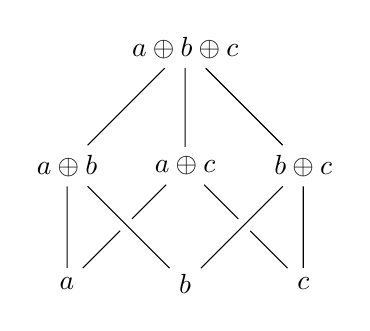
\begin{tikzpicture}
  \node (max) at (0,3) {$a\oplus b\oplus c$};
  \node (a) at (-1.5,1.5) {$a\oplus b$};
  \node (b) at (0,1.5) {$a\oplus c$};
  \node (c) at (1.5,1.5) {$b\oplus c$};
  \node (d) at (-1.5,0) {$a$};
  \node (e) at (0,0) {$b$};
  \node (f) at (1.5,0) {$c$};
  \draw	(d) -- (a) -- (max) -- (b) -- (f)
 			(f) -- (c) -- (max)
  			(d) -- (b);
  \draw[preaction={draw=white, -,line width=6pt}] (a) -- (e) -- (c);
\end{tikzpicture}
\end{figure}

In the same way as mentioned above, denotation \REF{defsem} gives rise to maximal interpretation. For example, the denotation can introduce the interpretation in \REF{PossNum} that Dima has exactly five books (`$a\oplus b\oplus c\oplus d\oplus e$', each atom of which is a book in this case) because of \cnst{max}.

As a result of the discussion presented so far, I hypothesize that the contrast in interpretations between \REF{NumPoss}/\REF{NumPoss2} and \REF{PossNum}/\REF{PossNum2} can be reduced to the simple difference in definiteness without any relation to the syntactic position of the possessors.

In \sectref{secDE} and \sectref{secGN}, I show that the hypothesis presented in this section is valid through tests using the definiteness effect and the genitive of negation as diagnostics.

\section{Test 1: The definiteness effect}\label{secDE}
\subsection{The definiteness effect}

Restrictions regarding the syntactic distribution of definites and indefinites are termed the \textsc{definiteness effect} (DE; also known as definiteness restriction). DE can be observed in a number of constructions in various languages.

Thus, for instance, subjects of English existential \textit{there}-sentences are known to be limited to indefinite nouns as shown in \REF{en}.

\ea \label{en}
\ea[]{There was a table in the garden.}
\ex[*]{There was the table in the garden.}
\z\z

\noindent In Icelandic, direct objects can be shifted before negative markers in some cases. As \REF{ice1} and \REF{ice2} illustrate, the definite direct object undergoes object shift but the indefinite one does not.

\ea\label{ice1}
    \ea
    \gll	Jón las ekki \minsp{[} bækurnar].\\
		John read \textsc{neg} {} books.\textsc{def}\\
    \ex
    \gll	Jón las \minsp{[} bækurnar] ekki.\\
		John read {} books.\textsc{def} \textsc{neg}\\
	\z
\glt	`John did not read the books.' \hfill (Icelandic; \citealt[392]{Collins.Thrainsson1996}) \\
\z

\ea\label{ice2}
\ea[]{\gll Hann las ekki \minsp{[} bækur].\\
he read \textsc{neg} {} books\\}
\ex[*]{\gll	Hann las \minsp{[} bækur] ekki.\\
he read {} books \textsc{neg}\\}
    \z
\glt `He didn't read books.' \hfill (Icelandic; \citealt[24]{Ritter.Rosen2005})
\z

\noindent In Hebrew, only the definite direct object is overtly marked for accusative case, whereas the indefinite one is not; see \REF{heb}.

\ea \label{heb}
\ea \gll ani karati et ha-sefer.\\
I read \textsc{acc} \textsc{def}-book\\
\glt `I read the book.'
\ex
\gll	ani karati \minsp{(*} et) sefer.\\
I read {} \textsc{acc} book\\
\glt	`I read a book.'
\hfill (Hebrew; \citealt[24]{Ritter.Rosen2005})
\z\z

\subsection{DE in Russian}

\citet{Paducheva2000} points out that a DE similar to English also exists in Russian existential constructions; cf. the sentences in \REF{enre} and \REF{rudef}, respectively.

\ea\label{enre}
\ea[]{\label{enre1} There is a pig in the garden.}
\ex[]{\label{enre2} There were three sailors standing on the corner.}
\ex[]{\label{enre3} There are many solutions to this problem.}
\ex[?]{\label{enre4} There is every tiger in the garden.}
\ex[?]{\label{enre5} There were most students in the hall.}
\ex[?]{\label{enre6} There are all solutions to this problem. \hfill \citep[58]{Bach1989}}
\z
\z

\ea\label{rudef}
\ea[]{\label{rudef1}
\gll V ogorode svinja. / V ogorode est' svinja.\\
in garden.\textsc{loc} pig.\textsc{nom.sg} {} in garden.\textsc{loc} is pig.\textsc{nom.sg}\\
\glt `There is a pig in the garden.'}
\ex[]{\label{rudef2}
\gll	Na uglu stojat {} tri matrosa.\\
on corner.\textsc{loc} stand \minsp{[} three sailors].\textsc{nom}\\
\glt `There are three sailors standing on the corner.'}
\ex[]{\label{rudef3}
\gll	\minsp{\{} Est' / Suščestvuet\} {} mnogo rešenij  {} ėtoj problemy. \\
{} is {} exists \minsp{[} many solutions].\textsc{nom} \minsp{[} this problem].\textsc{gen.sg}\\
\glt `There are many solutions to this problem.'}
\ex[*]{\label{rudef4}
\gll	V sadu est' {} každyj tigr.\\
in garden.\textsc{loc} is \minsp{[} every tiger].\textsc{nom.sg}\\
\glt Intended: `There is every tiger in the garden.'}
\ex[*]{\label{rudef5}
\gll	V auditorii bylo bol'šinstvo studentov.\\
in hall.\textsc{loc} was majority.\textsc{nom.sg} student.\textsc{gen.pl}\\
\glt Intended: `There were most students in the lecture hall.'}
\ex[*]{\label{rudef6}
\gll	\minsp{\{} Est' / Suščestvujut\} {} vse rešenija {} ėtoj problemy.\\
{} are {} exist \minsp{[} all solution].\textsc{nom.pl} \minsp{[} this problem].\textsc{gen.sg}\\
\glt Intended: `There are all solutions to this problem.'}
\z
\hfill \citep[134]{Paducheva2000}
\z

\noindent The Russian sentences in \REF{rudef} are grammatical if the corresponding English sentences in \REF{enre} are also grammatical as is shown in \REF{enre1}--\REF{enre3} and \REF{rudef1}--\REF{rudef3}, respectively. Likewise, Russian sentences are ungrammatical if the corresponding English sentences display low acceptability as in \REF{enre4}--\REF{enre6} and \REF{rudef4}--\REF{rudef6}, respectively. The Russian translations preserve the (un)grammaticality in their English counterparts regarding DE in existential constructions.\footnote{There are some differences regarding DE between English and Russian as shown in \REF{john-engl} and \REF{Dzon}.
    \ea\label{john-engl}
	\ea[*]{There wasn't John at the party.}
	\ex[*]{There weren't John's ten students at the party.
	\hfill \citep[69]{Keenan1996}}
	\z\z

	\ea\label{Dzon}
	\ea
	\gll	Na večere ne bylo Džona.\\
	at party.\textsc{loc} \textsc{neg} was John.\textsc{gen}\\
	\glt `John wasn't at the party.'
	\ex
	\gll	Na večere ne prisutstvovali {} vse desjat' aspirantov Džona.\\
	at party.\textsc{loc} \textsc{neg} were.present \minsp{[} all ten graduate.student].\textsc{nom} John.\textsc{gen}\\
	\glt `Not all John's ten students were at the party.'
	\\ \hfill \citep[134-135]{Paducheva2000}
	\z\z
    \noindent The ungrammaticality in the English sentences in \REF{john-engl} is not preserved in their Russian translations in \REF{Dzon}. \citet{Paducheva2000} attributes the difference in grammaticality to lexical differences between the existential verb \textit{byt'} in Russian and \textit{to be} in English. It should be noted that these are negated sentences.}

\subsection{Test by DE}\label{sec:testDE}

The Russian DE in the existential construction can be used as a test to verify validity of my hypothesis that the contrast in interpretations between \REF{NumPoss}, \REF{NumPoss2} and \REF{PossNum}, \REF{PossNum2} can be reduced to the difference in definiteness.

Phrases without maximal interpretation like \REF{NumPoss} and \REF{NumPoss2} can occur in the existential construction without any problem as demonstrated in \REF{DEnumposs} and \REF{DEnumposs2}, whereas phrases with maximal interpretation like \REF{PossNum} and \REF{PossNum2} are semantically odd as shown in \REF{DEpossnum} and \REF{DEpossnum2}.

%    \largerpage[-1] % Have all of (22) on next page

\ea \label{DE} \REF{NumPoss} and \REF{PossNum} in the existential construction
\ea[]{\label{DEnumposs}
\gll	V {knižnom škafu} est' pjat' Diminyx knig.\\
		in bookshelf.\textsc{loc} are five Dima's.\textsc{gen.pl} book.\textsc{gen.pl}\\
		\glt	`There are five of Dima's books in the bookshelf.'}
\ex[\#]{\label{DEpossnum}
\gll	V {knižnom škafu} est' Diminy pjat' knig\\
		in bookshelf.\textsc{loc} are Dima's.\textsc{nom.pl} five book.\textsc{gen.pl}\\
		\glt `There are Dima's five books in the bookshelf.'}
\z\z

\ea\label{DE2} \REF{NumPoss2} and \REF{PossNum2} in the existential construction
\ea[]{\label{DEnumposs2}
\gll	Na polu est' devjat' Mašinyx sumok.\\
		on floor.\textsc{loc} are nine Masha's.\textsc{gen.pl} bag.\textsc{gen.pl}\\
		\glt	`There are nine bags of Masha's on the floor.'}
\ex[\#]{\label{DEpossnum2}
\gll	Na polu est' Mašiny devjat' sumok\\
		on floor.\textsc{loc} are Masha's.\textsc{nom.pl} nine bag.\textsc{gen.pl}\\
		\glt `There are Masha's nine bags on the floor.'}
\z\z

\noindent The (un)acceptability of the sentences in \REF{DE} and \REF{DE2} is indicative that what lies behind the semantic oddity of \REF{PossNum} and \REF{PossNum2} is the fact that definite NPs are in general excluded from the existential construction both in Russian and English. Accordingly, \REF{PossNum} and \REF{PossNum2} are definite, while \REF{NumPoss} and \REF{NumPoss2} are indefinite.

Note, moreover, that phrases with adnominal genitives as possessors as in \REF{Num-Gen} can be interpreted either maximally or non-maximally, which is why they can occur in the existential construction as demonstrated in \REF{DE-GEN}.
    \ea\label{DE-GEN}\REF{Num-Gen} in the existential construction
	\ea\label{DEgen}
	\gll	V {knižnom škafu} est' pjat' knig Dimy.\\
	    	in bookshelf.\textsc{loc} are five book.\textsc{gen.pl} Dima.\textsc{gen}\\
	\glt	`There are five of Dima's books in the bookshelf.'
	\ex\label{DEgen2}
	\gll	Na polu est' devjat' sumok Maši.\\
			on floor.\textsc{loc} are nine bag.\textsc{gen.pl} Masha.\textsc{gen}\\
	\glt	`There are nine bags of Masha's on the floor.'
	\z\z

\noindent I claim that both \textit{pjat' knig Dimy} and \textit{devjat' sumok Maši} have to be interpreted non-maximally in order to avoid semantic oddity.

\section{Test 2: The genitive of negation}\label{secGN}

\subsection{The genitive of negation}

The genitive of negation (GN), which is available in several Slavic languages, is a phenomenon where an argument is marked with generative case under sentential negation although the argument is marked with the nominative or accusative case in a corresponding affirmative sentence.\footnote{Sometimes not only arguments but also adjuncts bear genitive case due to GN. For the sake of simplicity, this paper addresses GN on verbal arguments only.}

While the case alternation between nominative and genitive occurs on subjects of unaccusative verbs as shown in \REF{GN-S},\footnote{In addition to subjects of unaccusatives, GN can also appear on subjects of passive predicates under sentential negation.
%, which is shown in \REF{pass}.
%    \ea\label{pass}
%    \ea \gll Ėta kniga byla pročitana neskol'ko raz.\\
%        this book.\textsc{nom} was read several times\\
%    \glt `This book was read several times.'
%    \ex \gll Nikakix knig ne bylo pročitano.\\
%        no books.\textsc{gen} \textsc{neg} were read\\
%    \glt `No books were read.' \hfill \citep[651]{Harves2002}
%    \z\z
    %\noindent On the other hand, the case alternation does not occur on subjects of transitive and unergative verbs.
%    \ea
%    \ea\label{trn} Transitive subjects\\
%    \gll \{ Nikto / \minsp{*} Nikogo\ \} ne čitaet ėtu knigu.\\
%       {} Nobody.\textsc{nom} {} {} Nobody.\textsc{gen} \textsc{neg} reads that book.\textsc{acc}\\
%    \glt `Nobody is reading that book.'
%    \ex \label{une} Unergative subjects\\
%    \gll \{ Nikakie devočki / \minsp{*} Nikakix devoček\ \} ne tancevali.\\
%    {} no girls.\textsc{nom} {} {} no girls.\textsc{gen} \textsc{neg} danced\\
%    \glt `No girls danced.' \hfill \citep[651]{Harves2002}
%    \z\z
}
the alternation between accusative and genitive case occurs on direct objects of transitive verbs as shown in \REF{GN-O}.\footnote{Some researchers (e.g., \citealp{Peskovskij1956,Pesetsky1982,Franks1995,Borovikoff1997,Szucsich2001,Bailyn2012}) point out that the case alternation can occur on specific accusative nominal adverbials.
    %; see \REF{xii}.
    %\ea\label{xii}
    %\ea
    %\gll Boris ne putešestvoval i \{ nedelju / nedeli\ \}.\\
    %    Boris.\textsc{nom} \textsc{neg} even {} {} week.\textsc{acc} {} week.\textsc{gen}\\
    %\glt `Boris did not travel for even a week.'
    %\ex
    %\gll Sveta ne vela mašinu i \{ kilometr / kilometra\ \}.\\
    %    Sveta.\textsc{nom} \textsc{neg} drove car.\textsc{acc} even {} kilometer.\textsc{acc} {} kilometer.\textsc{gen}\\
    %\glt `Sveta did not drive the car even a kilometer.' \hfill \citep[67]{Borovikoff1997}
    %\z\z
However, there is debate about whether the genitive case on this type of adjuncts is an instance of the partitive genitive \citep[see][]{Franks.Dziwirek1993} rather than the GN \citep[see][]{Borovikoff1997,Pereltsvaig2000}.
}

\ea\label{GN-S}
\ea\label{GN-SN}
\gll	Pis'mo ne prišlo.\\
	letter.\textsc{nom} \textsc{neg} came\\
\glt	`The letter did not come.'
\ex\label{GN-SG}
\gll	Pis'ma ne prišlo.\\
	letter.\textsc{gen} \textsc{neg} came\\
\glt	`A letter did not come. (No letter came.)'
\hfill \citep[292]{Apresjan1985}
\ex\label{GN-Saf}
\gll	\minsp{\{} Pis'mo / \minsp{*} Pis'ma\} prišlo.\\
	{} letter.\textsc{nom} {} {} letter.\textsc{gen} came\\
\glt	`A/The letter came.'
\z\z

\ea\label{GN-O}
\ea\label{GN-OA}
\gll	Anna ne kupila žurnal.\\
	Anna.\textsc{nom} \textsc{neg} bought magazine.\textsc{acc}\\
\glt `Anna did not buy the magazine.'

\ex\label{GN-OG}
\gll	Anna ne kupila žurnala.\\
	Anna.\textsc{nom} \textsc{neg} bought magazine.\textsc{gen}\\
\glt	`Anna did not buy a magazine.'

\ex\label{GN-Oaf}
\gll	Anna kupila \minsp{\{} žurnal / \minsp{*} žurnala\}.\\
	Anna.\textsc{nom} bought {} magazine.\textsc{acc} {} {} magazine.\textsc{gen}\\
\glt	`Anna bought a/the magazine.'
\hfill \citep[647]{Harves2002}
\z\z

\noindent The nominative-case subject in \REF{GN-SN} can be altered with the genitive-case subject in \REF{GN-SG} under sentential negation. In the same way, the accusative-case direct object in \REF{GN-OA} can be exchanged with the genitive-case object in \REF{GN-OG}. Crucially, these alternations do not occur in affirmative sentences.

Many syntactic and semantic (and sometimes stylistic) factors affect the choice between genitive and nominative/accusative. What is significant for this paper is that genitive arguments are generally interpreted as indefinite/non-specific, while accusative arguments tend to be interpreted as definite/specific (see, a.o., \citealt{Timberlake1975,Harves2002,Kim2003,Partee.Borschev2004,Kagan2012,Harves2013}).

\subsection{Test by GN}

In order to verify the validity of my hypothesis that the contrast in interpretation between non-maximal \REF{NumPoss}/\REF{NumPoss2} and maximal \REF{PossNum}/\REF{PossNum2} can be reduced to the differences in definiteness, GN can be used as a test in the same way as DE, since GN is likewise sensitive to definiteness.\footnote{It is certain that the determinant of GN cannot be reduced to definiteness even if the focus is limited to the case alternation between genitive and accusative on direct objects. See, among many others, \citet{Timberlake1975}, \citet{Kagan2012}, and \cite{Geist2015} for the discussion of possible alternative and additional factors.
%For example, \citet{Kagan2012} shows that the following semantic factors except definiteness affect the choice of case: \textit{abstract/concrete, number, proper/common, specificity and scope}. Furthermore, \citet{Timberlake1975} lists more factors:
%    \textit{mass/count, inanimate/animate, emphatic negation/neutral, neutral/topicalized, unmodified/modified, finite/infinitive, imperfective/perfective} and so on. \cite{Geist2015} investigates this phenomena from the perspectives of situation semantics and concludes that more important factors for determining whether alternation occurs is not so much definiteness as event (in)dependency of the respective NP in situational semantics. Following \cite{Geist2015}, under negation, \textsc{acc} NPs are event independent and related to the free situation variable introduced by their determiner. In contrast, \textsc{gen} NPs are event dependent and related to the bound situation variable associated with the event argument introduced by the main predicate. As shown above, it is challenging to reveal the exact conditions under which the case alternation is allowed. However, a commonly adopted generalization is that the \textsc{acc} is associated with a definite interpretation and that the \textsc{gen} is associated with an indefinite interpretation. The definiteness is one of the big factors displaying correlation with GN. Thus, I use GN to test the hypothesis in this section. The result of the test may not lead to direct evidence as long as some factors except definiteness may affect the case alternation, but it is significant at least as collateral evidence.
}

Phrases with a non-maximal interpretation like \REF{NumPoss} and \REF{NumPoss2} readily occur in GN environments as demonstrated in \REF{GNnumposs} and \REF{GNnumposs2}, respectively. On the other hand, phrases with a maximal interpretation like \REF{PossNum} and \REF{PossNum2} result in semantic oddity as illustrated in \REF{GNpossnum} and \REF{GNpossnum2}, respectively.

%    \largerpage

\ea \label{GN} \REF{NumPoss} and \REF{PossNum} in the environment of GN
\ea[]{\label{GNnumposs}
\gll	Ivan ne čital {} pjati Diminyx knig.\\
		Ivan.\textsc{nom} \textsc{neg} read \minsp{[} five Dima's books].\textsc{gen}\\}
\ex[\#]{\label{GNpossnum}
\gll	Ivan ne čital {} Diminyx pjati knig.\\
	    Ivan.\textsc{nom} \textsc{neg} read \minsp{[} Dima's five books].\textsc{gen}\\
	    \glt    `Ivan did not read five of Dima's books.'}
\z\z

\ea\label{GN2} \REF{NumPoss2} and \REF{PossNum2} in the environment of GN
\ea[]{\label{GNnumposs2}
\gll	 Ja ne bral {} devjati Mašinyx sumok.\\
	 I.\textsc{nom} \textsc{neg} took \minsp{[} nine Masha's bags].\textsc{gen}\\}
\ex[\#]{\label{GNpossnum2}
\gll	Ja ne bral {} Mašinyx devjati sumok.\\
	    I.\textsc{nom} \textsc{neg} took \minsp{[} Masha's nine bags].\textsc{gen}\\
	 \glt   `I did not take nine of Masha's bags.'}
\z\z

\noindent Moreover, the phrases interpreted non-maximally render the acceptability of the sentence lower if they occur as accusative objects under sentential negation as is shown in \REF{NegAnumposs} and \REF{NegAnumposs2}, respectively. In contrast, the phrases with a maximal interpretation are grammatical in the same environment; see \REF{NegApossnum} and \REF{NegApossnum2}.

\ea \label{NegA} \REF{NumPoss} and \REF{PossNum} as accusative objects in a negated environment
\ea[??]{\label{NegAnumposs}
\gll    Ivan ne čital {} pjat' Diminyx knig.\\
		Ivan.\textsc{nom} \textsc{neg} read \minsp{[} five Dima's books].\textsc{acc}\\}
\ex[\phantom{??}]{\label{NegApossnum}
\gll	Ivan ne čital {} Diminy pjat' knig.\\
		Ivan.\textsc{nom} \textsc{neg} read \minsp{[} Dima's five books].\textsc{acc}\\
\glt	`Ivan did not read Dima's five books.'}
\z\z

\ea \label{NegA2} \REF{NumPoss2} and \REF{PossNum2} as accusative objects in a negated environment
\ea[??]{\label{NegAnumposs2}
\gll    Ja ne bral {} devjat' Mašinyx sumok.\\
	    I.\textsc{nom} \textsc{neg} took \minsp{[} nine Masha's bags].\textsc{acc}\\}
\ex[\phantom{??}]{\label{NegApossnum2}
\gll	Ja ne bral {} Mašiny devjat' sumok.\\
	I.\textsc{nom} \textsc{neg} took \minsp{[} Masha's nine bags].\textsc{acc}\\
\glt	`I did not take Masha's nine bags.'}
\z\z

\noindent The facts shown in \REF{GN}--\REF{NegA2} suggest that the phrases in \REF{PossNum} and \REF{PossNum2}, which are interpreted maximally, are definite, while the phrases interpreted non-maximally in \REF{NumPoss} and \REF{NumPoss2} are indefinite, since arguments in genitive case are interpreted as indefinite, while arguments in the accusative case are interpreted as definite.

%\footnote{As already pointed out in %footnote \ref{fn:adnominal.poss}
%\sectref{sec:testDE}, phrases as \REF{Num-Gen}, where adnominal genitives are used as possessors, can be interpreted either maximally or non-maximally. It follows that they can occur both as a \textsc{gen} objects and as \textsc{acc} objects under sentential negation. I claim that the relevant \textsc{gen} objects have to receive a non-maximal interpretation, whereas the relevant \textsc{acc} objects have to be interpreted maximally in order to avoid semantic oddity.
%	\ea \label{GN-GEN} \REF{Num-Gen} in the environment of GN
%	\ea
%	\gll	Ivan ne čital {} pjati knig Dimy.\\
%	        Ivan.\textsc{nom} \textsc{neg} read \minsp{[} five books Dima.\textsc{gen.pl}]\\
%	\glt	`Ivan did not read five of Dima's books.'

%\ex
%	\gll	 Ja ne bral {} devjati sumok Maši.\\
%			 I.\textsc{nom} \textsc{neg} took \minsp{[} nine bags Masha.\textsc{gen}]\\
%	\glt	`I did not take nine of Masha's bags.'
%	\z\z

%	\ea \label{NegA-GEN} \REF{Num-Gen} as an \textsc{acc} object in the negative environment
%	\ea
%	\gll	Ivan ne čital {} pjat' knig Dimy.\\
%			Ivan.\textsc{nom} \textsc{neg} read \minsp{[} five books Dima.\textsc{gen}].\textsc{acc}\\
%	\glt	`Ivan did not read Dima's five books.'

%	\ex
%	\gll	Ja ne bral {} devjat' sumok Maši.\\
%			I.\textsc{nom} \textsc{neg} took \minsp{[} nine bags Masha.\textsc{gen}].\textsc{acc}\\
%	\glt	`I did not take Masha's nine bags.'
%	\z\z
%	}

\section{Conclusion}\label{CON}

I have provided some data regarding non-/maximal interpretation and demonstrated that the relevant interpretation of nominal phrases arises independently of the syntactic position of the possessor. That is, the maximal interpretation comes about not only through high possessors (possessive adjectives and pronouns) but also through low possessors (adnominal genitives). Therefore, the maximal interpretation of nominal phrases cannot be used as a diagnostic to support the existence of DP projections in Russian. In addition, I have shown that the contrast between the maximal and non-maximal interpretations can be reduced to the difference between definiteness and indefiniteness by means of the tests of definiteness effect and genitive of negation.

It goes without saying that there are many other issues left regarding definiteness and the syntactic structure of Russian nominal phrases. I believe, however, that the present paper makes a small contribution to the resolution of these issues.

\section*{Abbreviations}
\begin{tabularx}{.5\textwidth}{@{}lX@{}}
\textsc{acc} & accusative case\\
DE & definiteness effect\\
\textsc{def} & definite article\\
\textsc{gen} & genitive case\\
GN & genitive of negation\\
\end{tabularx}%
\begin{tabularx}{.5\textwidth}{@{}lX@{}}
\textsc{loc} & locative case\\
\textsc{neg} & negation\\
\textsc{nom} & nominative case\\
\textsc{pl} & plural\\
\textsc{sg} & singular\\
\end{tabularx}

\section*{Acknowledgements}
An earlier version of this paper has been presented at the workshop ``Semantics of Noun Phrases'' which was part of FDSL 13 at the University of Göttingen (at that time I was affiliated with the Tokyo University of Foreign Studies and the Japan Society for the Promotion of Science). I am very grateful to the participants of the workshop for helpful discussion. I would like to thank two anonymous reviewers for their valuable comments. I also appreciate the contribution of the native speakers who assessed my Russian data. All misunderstandings and errors remain my own. The research reported here was supported by JSPS Grants-in-Aid for Scientific Research (\#17J07534, \#19K23073, PI: Takuya Miyauchi).

\sloppy
\printbibliography[heading=subbibliography,notkeyword=this]

\end{document}
